\batchmode
\documentclass[a4paper]{book}
\usepackage{a4wide}
\usepackage{makeidx}
\usepackage{graphicx}
\usepackage{multicol}
\usepackage{float}
\usepackage{listings}
\usepackage{color}
\usepackage{textcomp}
\usepackage{alltt}
\usepackage{times}
\usepackage{ifpdf}
\ifpdf
\usepackage[pdftex,
            pagebackref=true,
            colorlinks=true,
            linkcolor=blue,
            unicode
           ]{hyperref}
\else
\usepackage[ps2pdf,
            pagebackref=true,
            colorlinks=true,
            linkcolor=blue,
            unicode
           ]{hyperref}
\usepackage{pspicture}
\fi
\usepackage[utf8]{inputenc}
\usepackage{doxygen}
\lstset{language=C++,inputencoding=utf8,basicstyle=\footnotesize,breaklines=true,breakatwhitespace=true,tabsize=1,numbers=left }
\makeindex
\setcounter{tocdepth}{3}
\renewcommand{\footrulewidth}{0.4pt}
\begin{document}
\hypersetup{pageanchor=false}
\begin{titlepage}
\vspace*{7cm}
\begin{center}
{\Large Media \\[1ex]\large 0.01 }\\
\vspace*{1cm}
{\large Generated by Doxygen 1.6.3}\\
\vspace*{0.5cm}
{\small Wed May 19 21:31:09 2010}\\
\end{center}
\end{titlepage}
\clearemptydoublepage
\pagenumbering{roman}
\tableofcontents
\clearemptydoublepage
\pagenumbering{arabic}
\hypersetup{pageanchor=true}
\chapter{Data Structure Index}
\input{annotated}
\chapter{File Index}
\section{File List}
Here is a list of all files with brief descriptions:\begin{DoxyCompactList}
\item\contentsline{section}{\hyperlink{main_8c}{main.c} }{\pageref{main_8c}}{}
\item\contentsline{section}{\hyperlink{main_8h}{main.h} }{\pageref{main_8h}}{}
\item\contentsline{section}{\hyperlink{media_8c}{media.c} }{\pageref{media_8c}}{}
\item\contentsline{section}{\hyperlink{media_8h}{media.h} }{\pageref{media_8h}}{}
\end{DoxyCompactList}

\chapter{Data Structure Documentation}
\input{struct_media_args}
\chapter{File Documentation}
\hypertarget{main_8c}{
\section{main.c File Reference}
\label{main_8c}\index{main.c@{main.c}}
}
{\ttfamily \#include $<$stdio.h$>$}\par
{\ttfamily \#include $<$stdlib.h$>$}\par
{\ttfamily \#include \char`\"{}media.h\char`\"{}}\par
Include dependency graph for main.c:\nopagebreak
\begin{figure}[H]
\begin{center}
\leavevmode
\includegraphics[width=82pt]{main_8c__incl}
\end{center}
\end{figure}
This graph shows which files directly or indirectly include this file:\nopagebreak
\begin{figure}[H]
\begin{center}
\leavevmode
\includegraphics[width=55pt]{main_8c__dep__incl}
\end{center}
\end{figure}
\subsection*{Defines}
\begin{DoxyCompactItemize}
\item 
\#define \hyperlink{main_8c_ab0139008fdda107456f13f837872b410}{PATH}~\char`\"{}/Users/bilalh/Movies/.Movie/mov/\char`\"{}
\end{DoxyCompactItemize}
\subsection*{Functions}
\begin{DoxyCompactItemize}
\item 
int \hyperlink{main_8c_abf9e6b7e6f15df4b525a2e7705ba3089}{main} (int argc, char const $\ast$argv\mbox{[}$\,$\mbox{]})
\end{DoxyCompactItemize}


\subsection{Define Documentation}
\hypertarget{main_8c_ab0139008fdda107456f13f837872b410}{
\index{main.c@{main.c}!PATH@{PATH}}
\index{PATH@{PATH}!main.c@{main.c}}
\subsubsection[{PATH}]{\setlength{\rightskip}{0pt plus 5cm}\#define PATH~\char`\"{}/Users/bilalh/Movies/.Movie/mov/\char`\"{}}}
\label{main_8c_ab0139008fdda107456f13f837872b410}


Definition at line 4 of file main.c.



\subsection{Function Documentation}
\hypertarget{main_8c_abf9e6b7e6f15df4b525a2e7705ba3089}{
\index{main.c@{main.c}!main@{main}}
\index{main@{main}!main.c@{main.c}}
\subsubsection[{main}]{\setlength{\rightskip}{0pt plus 5cm}int main (int {\em argc}, \/  char const $\ast$ {\em argv}\mbox{[}$\,$\mbox{]})}}
\label{main_8c_abf9e6b7e6f15df4b525a2e7705ba3089}


Definition at line 9 of file main.c.



Here is the call graph for this function:\nopagebreak
\begin{figure}[H]
\begin{center}
\leavevmode
\includegraphics[width=127pt]{main_8c_abf9e6b7e6f15df4b525a2e7705ba3089_cgraph}
\end{center}
\end{figure}



\hypertarget{main_8h}{
\section{main.h File Reference}
\label{main_8h}\index{main.h@{main.h}}
}

\hypertarget{media_8c}{
\section{media.c File Reference}
\label{media_8c}\index{media.c@{media.c}}
}
{\ttfamily \#include $<$Block.h$>$}\par
{\ttfamily \#include $<$dirent.h$>$}\par
{\ttfamily \#include $<$regex.h$>$}\par
{\ttfamily \#include $<$stdarg.h$>$}\par
{\ttfamily \#include $<$stdio.h$>$}\par
{\ttfamily \#include $<$stdlib.h$>$}\par
{\ttfamily \#include $<$strings.h$>$}\par
{\ttfamily \#include $<$sys/types.h$>$}\par
{\ttfamily \#include $<$unistd.h$>$}\par
{\ttfamily \#include \char`\"{}Media.h\char`\"{}}\par
Include dependency graph for media.c:\nopagebreak
\begin{figure}[H]
\begin{center}
\leavevmode
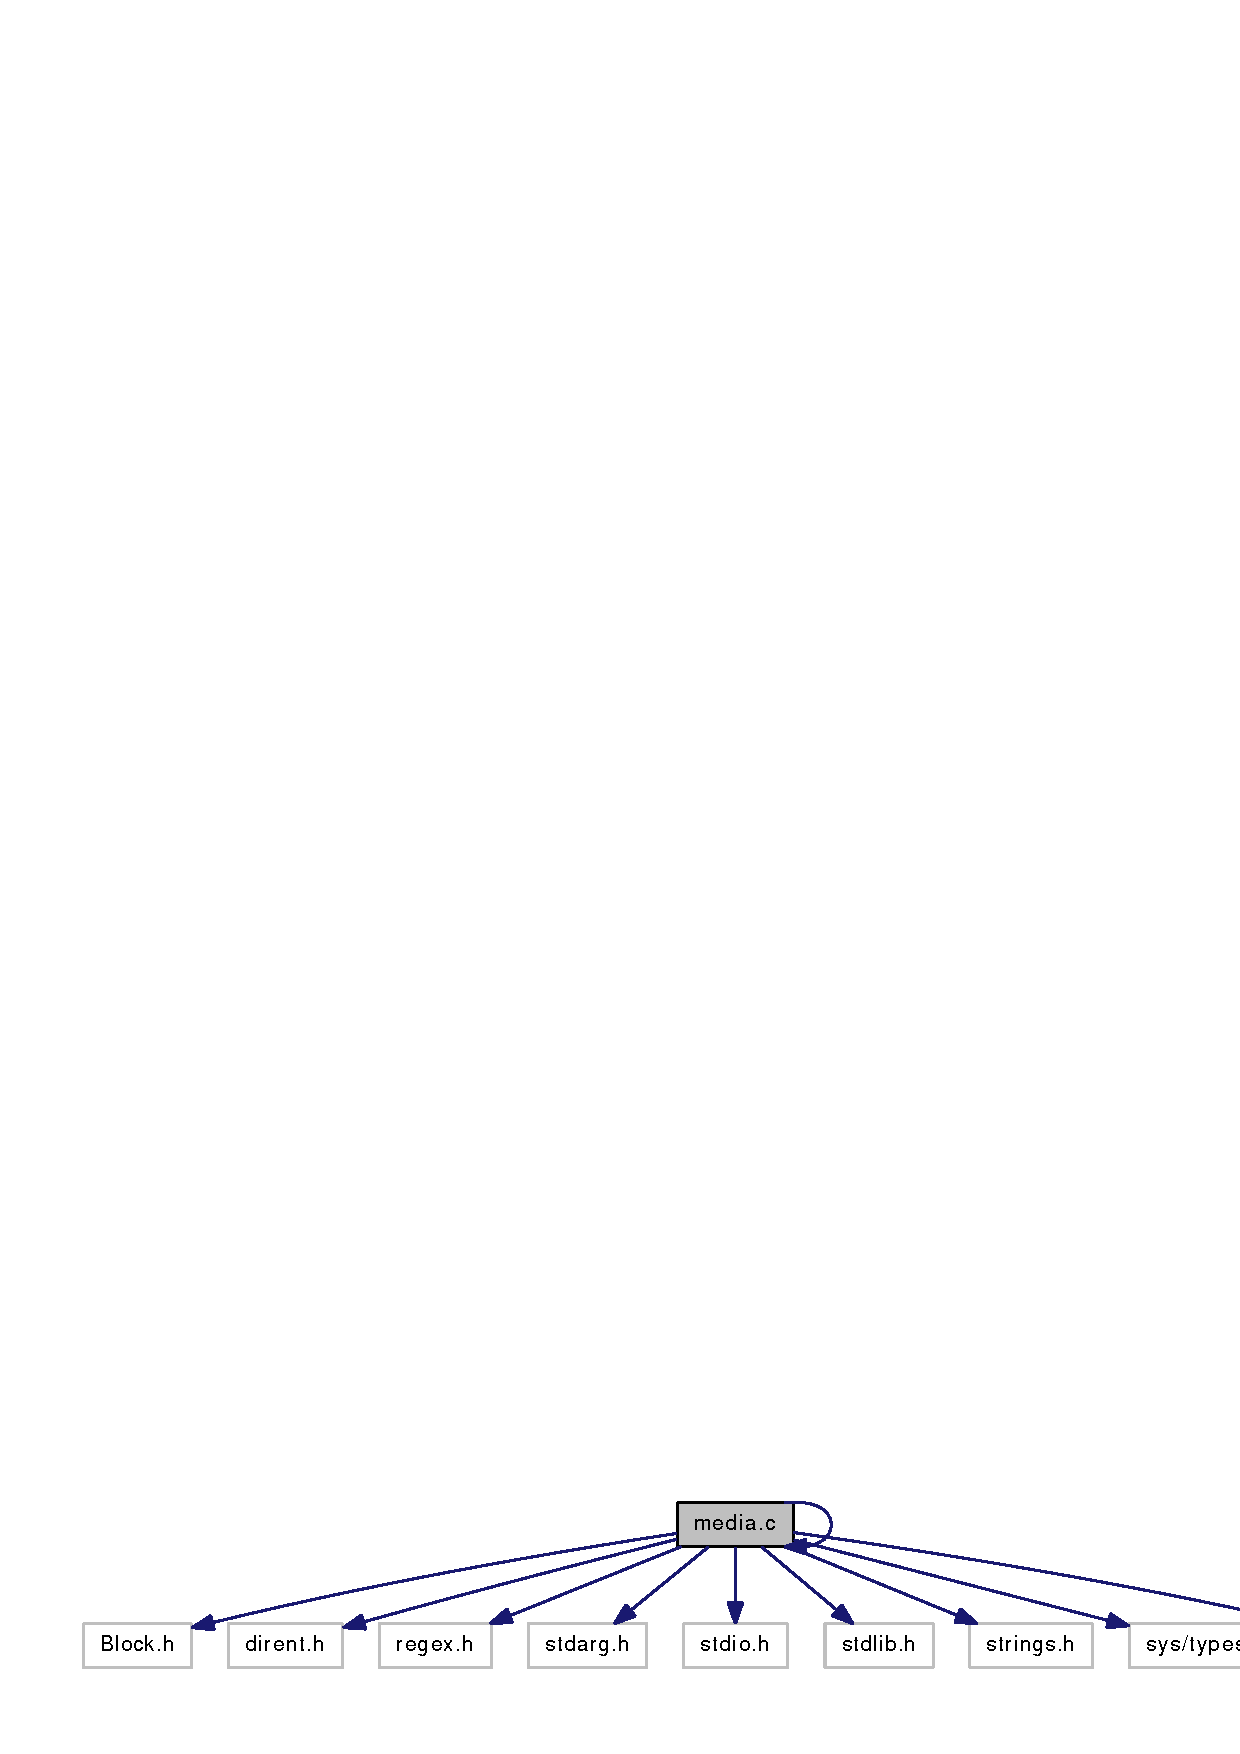
\includegraphics[width=347pt]{media_8c__incl}
\end{center}
\end{figure}
This graph shows which files directly or indirectly include this file:\nopagebreak
\begin{figure}[H]
\begin{center}
\leavevmode
\includegraphics[width=59pt]{media_8c__dep__incl}
\end{center}
\end{figure}
\subsection*{Defines}
\begin{DoxyCompactItemize}
\item 
\#define \hyperlink{media_8c_a605917f1cfa78dfcfae65ce2383e4aa4}{DIRENT}(value)~($\ast$(struct dirent $\ast$$\ast$) value)
\end{DoxyCompactItemize}
\subsection*{Functions}
\begin{DoxyCompactItemize}
\item 
void \hyperlink{media_8c_a769cab1fb67e28ee26663e632190fb2f}{media} (char $\ast$path)
\item 
int \hyperlink{media_8c_a613aaf9cf7b0a71ac4f620e013bc75fc}{match} (const char $\ast$string, char $\ast$pattern)
\begin{DoxyCompactList}\small\item\em 1 on match, 0 on any error s \item\end{DoxyCompactList}\end{DoxyCompactItemize}


\subsection{Define Documentation}
\hypertarget{media_8c_a605917f1cfa78dfcfae65ce2383e4aa4}{
\index{media.c@{media.c}!DIRENT@{DIRENT}}
\index{DIRENT@{DIRENT}!media.c@{media.c}}
\subsubsection[{DIRENT}]{\setlength{\rightskip}{0pt plus 5cm}\#define DIRENT(value)~($\ast$(struct dirent $\ast$$\ast$) value)}}
\label{media_8c_a605917f1cfa78dfcfae65ce2383e4aa4}


Definition at line 12 of file media.c.



\subsection{Function Documentation}
\hypertarget{media_8c_a613aaf9cf7b0a71ac4f620e013bc75fc}{
\index{media.c@{media.c}!match@{match}}
\index{match@{match}!media.c@{media.c}}
\subsubsection[{match}]{\setlength{\rightskip}{0pt plus 5cm}int match (const char $\ast$ {\em string}, \/  char $\ast$ {\em pattern})}}
\label{media_8c_a613aaf9cf7b0a71ac4f620e013bc75fc}


1 on match, 0 on any error s 

Match string against the extended regular expression in pattern, treating errors as no match.

Return 1 for match, 0 for no match. 

Definition at line 34 of file media.c.

\hypertarget{media_8c_a769cab1fb67e28ee26663e632190fb2f}{
\index{media.c@{media.c}!media@{media}}
\index{media@{media}!media.c@{media.c}}
\subsubsection[{media}]{\setlength{\rightskip}{0pt plus 5cm}void media (char $\ast$ {\em path})}}
\label{media_8c_a769cab1fb67e28ee26663e632190fb2f}


Definition at line 14 of file media.c.



Here is the call graph for this function:\nopagebreak
\begin{figure}[H]
\begin{center}
\leavevmode
\includegraphics[width=89pt]{media_8c_a769cab1fb67e28ee26663e632190fb2f_cgraph}
\end{center}
\end{figure}



\hypertarget{media_8h}{
\section{media.h File Reference}
\label{media_8h}\index{media.h@{media.h}}
}
\subsection*{Functions}
\begin{DoxyCompactItemize}
\item 
void \hyperlink{media_8h_a769cab1fb67e28ee26663e632190fb2f}{media} (char $\ast$path)
\item 
int \hyperlink{media_8h_a613aaf9cf7b0a71ac4f620e013bc75fc}{match} (const char $\ast$string, char $\ast$pattern)
\begin{DoxyCompactList}\small\item\em 1 on match, 0 on any error s \item\end{DoxyCompactList}\end{DoxyCompactItemize}


\subsection{Function Documentation}
\hypertarget{media_8h_a613aaf9cf7b0a71ac4f620e013bc75fc}{
\index{media.h@{media.h}!match@{match}}
\index{match@{match}!media.h@{media.h}}
\subsubsection[{match}]{\setlength{\rightskip}{0pt plus 5cm}int match (const char $\ast$ {\em string}, \/  char $\ast$ {\em pattern})}}
\label{media_8h_a613aaf9cf7b0a71ac4f620e013bc75fc}


1 on match, 0 on any error s 

Match string against the extended regular expression in pattern, treating errors as no match.

Return 1 for match, 0 for no match. 

Definition at line 34 of file media.c.

\hypertarget{media_8h_a769cab1fb67e28ee26663e632190fb2f}{
\index{media.h@{media.h}!media@{media}}
\index{media@{media}!media.h@{media.h}}
\subsubsection[{media}]{\setlength{\rightskip}{0pt plus 5cm}void media (char $\ast$ {\em path})}}
\label{media_8h_a769cab1fb67e28ee26663e632190fb2f}


Definition at line 14 of file media.c.



Here is the call graph for this function:\nopagebreak
\begin{figure}[H]
\begin{center}
\leavevmode
\includegraphics[width=89pt]{media_8h_a769cab1fb67e28ee26663e632190fb2f_cgraph}
\end{center}
\end{figure}



\include{option_parser_012_8c}
\include{option_parser_8c}
\include{option_parser_8h}
\include{test_8c}
\printindex
\end{document}
